\part[The Scala Ecosystem]{The Scala Ecosystem}
\section{The Web}
\begin{frame}{Official Scala Website}
\begin{center}
\link{http://www.scala-lang.org/}{http://www.scala-lang.org/}
\end{center}
Stuff you find there:
\begin{itemize}
  \item Scala download link
  \item Documentation
  \item Guides
  \item Support information
  \item News
  \item and so on\ldots
\end{itemize}
\end{frame}

\begin{frame}{Official Industry-oriented Website}
\begin{center}
\link{http://www.typesafe.com/}{http://www.typesafe.com/}
\end{center}
Typesafe is a combination of:
\begin{description}
\item[\link{http://www.scala-lang.org/}{Scala}] programming language
\item[\link{http://akka.io/}{Akka}] event-driven middleware
\item[\link{http://www.playframework.org/}{Play!}] web framework
\end{description}
\pause
Typesafe provides \link{http://www.typesafe.com/stack}{The Typesafe Stack}:
\begin{itemize}
\item Scala, Akka, Play!
\item Simple Build Tool (\link{http://www.scala-sbt.org/}{SBT})
\item \link{https://github.com/n8han/giter8}{giter8} (a command line tool to
apply templates defined on github)
\end{itemize}
\end{frame}

\begin{frame}{Official Community-driven Documentation Website}
\begin{center}
\link{http://docs.scala-lang.org/}{http://docs.scala-lang.org/}
\end{center}
Stuff you find there:
\begin{itemize}
  \item Guides
  \item Tutorials
  \item Glossary
  \item Cheat sheets
  \item Scala Improvement Process
  \item \link{http://docs.scala-lang.org/style/}{Style Guide}
  \item and so on\ldots
\end{itemize}
\end{frame}

\begin{frame}{Scala Wiki}
\begin{center}
\link{https://wiki.scala-lang.org}{https://wiki.scala-lang.org}
\end{center}
Stuff you find there:
\begin{itemize}
  \item \link{https://wiki.scala-lang.org/display/SW/Tools+and+Libraries}{Tools
  and Libraries}
  \item Twitter links
  \item User Groups
\end{itemize}
\end{frame}

\begin{frame}{Stack Overflow}
\begin{center}
\link{http://stackoverflow.com}{http://stackoverflow.com}
\end{center}
\begin{block}{What is Stack Overflow?}
Stack Overflow is a question \& answer site about programming questions.
\end{block}
Stuff you find / can do there:
\begin{itemize}
  \item \link{http://stackoverflow.com/tags/scala/info}{Stack Overflow Scala Tutorial!}
  \item search for questions
  \item ask questions
  \item answer questions ;)
  \item follow topics of interest
  \item earn reputation
\end{itemize}
\end{frame}

\pictureframe{Scala on Stack Overflow and Github}{resources/SOGithub.pdf}

\begin{frame}{Symbol Hound}
\begin{center}
\link{http://symbolhound.com/}{http://symbolhound.com/}
\end{center}
\begin{center}
\begin{block}{What is Symbol Hound?}
\emph{Symbol Hound} is a search engine for symbols.
\end{block}
\begin{center}
Scala has lots of \alert{symbols} but \highlight{none} of them are language
\highlight{keywords}\\
Scala has very few language \highlight{keywords} and \highlight{none} of them
are \alert{symbolic}
\end{center}
\end{center}
\end{frame}

\begin{frame}{Simply Scala}
\begin{center}
\link{http://www.simplyscala.com/}{http://www.simplyscala.com/}
\end{center}
\begin{block}{What is Simply Scala?}
\emph{Simply Scala} is an \highlight{interactive} Scala tutorial
\end{block}
\end{frame}

\section{IDEs}
\begin{frame}{The old school way}
This is how you get the ``stand-alone'' Scala edition:
\begin{enumerate}
  \item Go to
  \link{http://www.scala-lang.org/downloads}{http://www.scala-lang.org/downloads}
  \item Download one of the \highlight{Stable} Releases
  \item Extract the files from the archive
  \item Manually adjust the environment variable for the \highlight{Path} to
  point to the \highlight{ScalaHomeDirectory/bin} folder
\end{enumerate}
\end{frame}

\begin{frame}{The old school way}
This is what you get from the ``stand-alone'' Scala edition:
\begin{description}
  \item[scala] Scala's interactive shell (REPL)
  \item[scalac] The Scala compiler
  \item[fsc] The Fast Scala compiler (scalac, which always runs as a daemon in
  the background)
  \item[sbaz] The Scala Bazar (a small console application, which provides
  access to main Scala repositories)
\end{description}
\begin{center}
Start the terminal and type ``\highlight{sbaz help}'' to get started
\end{center}
\end{frame}

\begin{frame}{The eclipse Scala plugin}
\begin{center}
\link{http://scala-ide.org/}{http://scala-ide.org/}
\end{center}
\begin{center}
An extra Scala installation is \highlight{not} required for the Scala
plugin for eclipse to work!
\end{center}
The plugin gives you:
\begin{enumerate}
  \item Support for Mixed Scala/Java Projects
  \item Scala perspective
  \item Scala REPL, which runs inside of Eclipse
  \item Scala compiler
  \item Scala debugger
\end{enumerate}
\end{frame}

\begin{frame}{The IntelliJ IDEA Scala plugin}
\begin{center}
\link{http://blog.jetbrains.com/scala/}{http://blog.jetbrains.com/scala/}
\end{center}
\begin{center}
An extra Scala installation \alert{is} required for the Scala
plugin for IntelliJ IDEA to work!
\end{center}
\begin{center}
Get started \link{http://confluence.jetbrains.net/display/SCA/Getting+Started+with+IntelliJ+IDEA+Scala+Plugin}{here}
\end{center}
\begin{center}
Take a look at the \link{https://github.com/orfjackal/idea-sbt-plugin}{IDEA SBT
plugin} as well
\end{center}
\end{frame}

\begin{frame}{Simple Build Tool}
\begin{center}
\link{http://www.scala-sbt.org/}{http://www.scala-sbt.org/}
\end{center}
\begin{center}
Get started
\link{https://github.com/harrah/xsbt/wiki/Getting-Started-Setup}{here}
\end{center}
SBT gives you:
\begin{enumerate}
  \item Scala REPL
  \item Scala-scripted configuration luxury
  \item \highlight{Continous incremental compilation}
  \item Out of the box testing with Scala test frameworks
  \item Concise dependency management DSL
  \item and \link{http://www.scala-sbt.org/}{further benefits}
\end{enumerate}
\end{frame}

\begin{frame}{The Typesafe Stack}
\begin{center}
\link{http://www.typesafe.com/stack/download}{http://www.typesafe.com/stack/download}
\end{center}
\begin{center}
Get started \link{http://www.typesafe.com/resources/getting-started/}{here}
\end{center}
\end{frame}

\begin{frame}{Recommended setup}
\begin{enumerate}
  \item Install the \highlight{JVM}
  \item Install \highlight{eclipse}
  \item Install the \highlight{Scala plugin for eclipse}
  \item Install the \highlight{typesafe stack} (installs \highlight{SBT} and
  \highlight{g8})
  \item Use eclipse only as an \highlight{editor}
  \item Use SBT to \highlight{compile/run/build/test}
  \item Use SBT plugin for eclipse to \highlight{create} and \highlight{import}
  projects with SBT into eclipse (plugin installation instructions on the next
  slide)
\end{enumerate}
The only reason to install the stand-alone Scala edition is the REPL, but the
REPL can be accessed from either eclipse or SBT, which is more than enough.
\end{frame}

\begin{frame}[fragile]{SBT plugin for eclipse}
\begin{center}
\link{https://github.com/typesafehub/sbteclipse}{https://github.com/typesafehub/sbteclipse}
\end{center}
\begin{center}
\alert{Do not} download it, SBT will do it for you!
\end{center}
\begin{block}{How do I setup the SBT plugin for eclipse?}
\begin{enumerate}
  \item go to \lstinline!~!\highlight{/.sbt/} or create it yourself
  \item create \lstinline!~!/.sbt/\highlight{plugins/} folder
  \item create \lstinline!~!/.sbt/plugins/\highlight{build.sbt} file
  \item paste the following into \lstinline!~!\highlight{/.sbt/plugins/build.sbt} and save it
\end{enumerate}
\end{block}
\begin{exampleblock}{Code for copying and pasting}
\begin{small}
resolvers += Classpaths.typesafeResolver
\newline
\lstinline!// an EMPTY line here!
\newline
addSbtPlugin("com.typesafe.sbteclipse" \% "sbteclipse-plugin" \% "latest.release")
\end{small}
\end{exampleblock}
\end{frame}

\begin{frame}{Creating a project}
\begin{block}{How do I create a Scala project?}
\begin{enumerate}
  \item Create a folder for your project: \highlight{MyAwesomeProject}
  \item Create MyAwesomeProject/\highlight{build.sbt} file
  \item Paste the following into \highlight{MyAwesomeProject/build.sbt} and save it:\\
  \lstinline!name := "My Awesome Project"!
  \item Start a terminal and \highlight{cd} into \highlight{MyAwesomeProject}
  \item Start SBT by typing \highlight{sbt} and pressing enter
  \item Type in \highlight{eclipse} and press enter
  \item Start eclipse and \highlight{import} your project using
  the \highlight{Existing Projects into Workspace} option under the
  \highlight{General} category
  \item Find the \highlight{Project} menu item in the menu bar at the top of
  eclipse
  \item Remove the \highlight{checkmark \checkmark} from \highlight{Build
  Automatically}
\end{enumerate}
\end{block}
\end{frame}

\begin{frame}[fragile]{Simple guide for SBT}
\begin{block}{What can I do with SBT?}
\begin{description}
\item[console] starts the REPL
\item[compile] compiles your production code
\item[test-compile] compiles your production code and your test code
\item[test] \lstinline!compile + test:compile +! runs your tests
\item[run] compiles your production code, then searches for \lstinline!main!
methods in your production code and either runs your application or makes you
decide, which \lstinline!main! method to run
\end{description}
\end{block}
\pause
\begin{center}
\lstinline!~!command - \highlight{continuous execution} of the command
triggered on source change
\end{center}
\end{frame}

\section{Testing}
\begin{frame}[fragile]{Testing - ScalaTest}
\begin{center}
\link{http://www.scalatest.org/}{http://www.scalatest.org/}
\end{center}
\begin{lstlisting}[basicstyle=\scriptsize]
libraryDependencies += "org.scalatest" %% "scalatest" % "latest.release" % "test"
\end{lstlisting}
\begin{block}{What is ScalaTest?}
ScalaTest is an open-source test framework for the Java Platform designed to
increase your productivity by letting you write fewer lines of test code that
more clearly reveal your intent.
\end{block}
\end{frame}
\begin{frame}[fragile]{Testing - Specs2}
\begin{center}
\link{http://etorreborre.github.com/specs2/}{http://etorreborre.github.com/specs2/}
\end{center}
\begin{lstlisting}[basicstyle=\scriptsize]
libraryDependencies += "org.specs2" %% "specs2" % "latest.release" % "test"
\end{lstlisting}
\begin{block}{What is Specs2?}
Specs2 is a library for writing executable software specifications. With specs2
you can write software specifications for one class (unit specifications) or a
full system (acceptance specifications).
\end{block}
\end{frame}

\begin{frame}[fragile]{Testing - ScalaCheck}
\begin{center}
\link{http://code.google.com/p/scalacheck/}{http://code.google.com/p/scalacheck/}
\end{center}
\begin{lstlisting}[basicstyle=\scriptsize]
libraryDependencies += "org.scala-tools.testing" %% "scalacheck" % "latest.release" % "test"
\end{lstlisting}
\begin{block}{What is ScalaCheck?}
ScalaCheck is a powerful tool for automatic unit testing of Scala and Java
programs. It features automatic test case generation and minimization of failing
test cases. ScalaCheck started out as a Scala port of the Haskell library
QuickCheck, and has since evolved and been extended with features not found in
Haskell QuickCheck.
\end{block}
\end{frame}

\section{Literature}
\begin{frame}{Literature}
\begin{center}
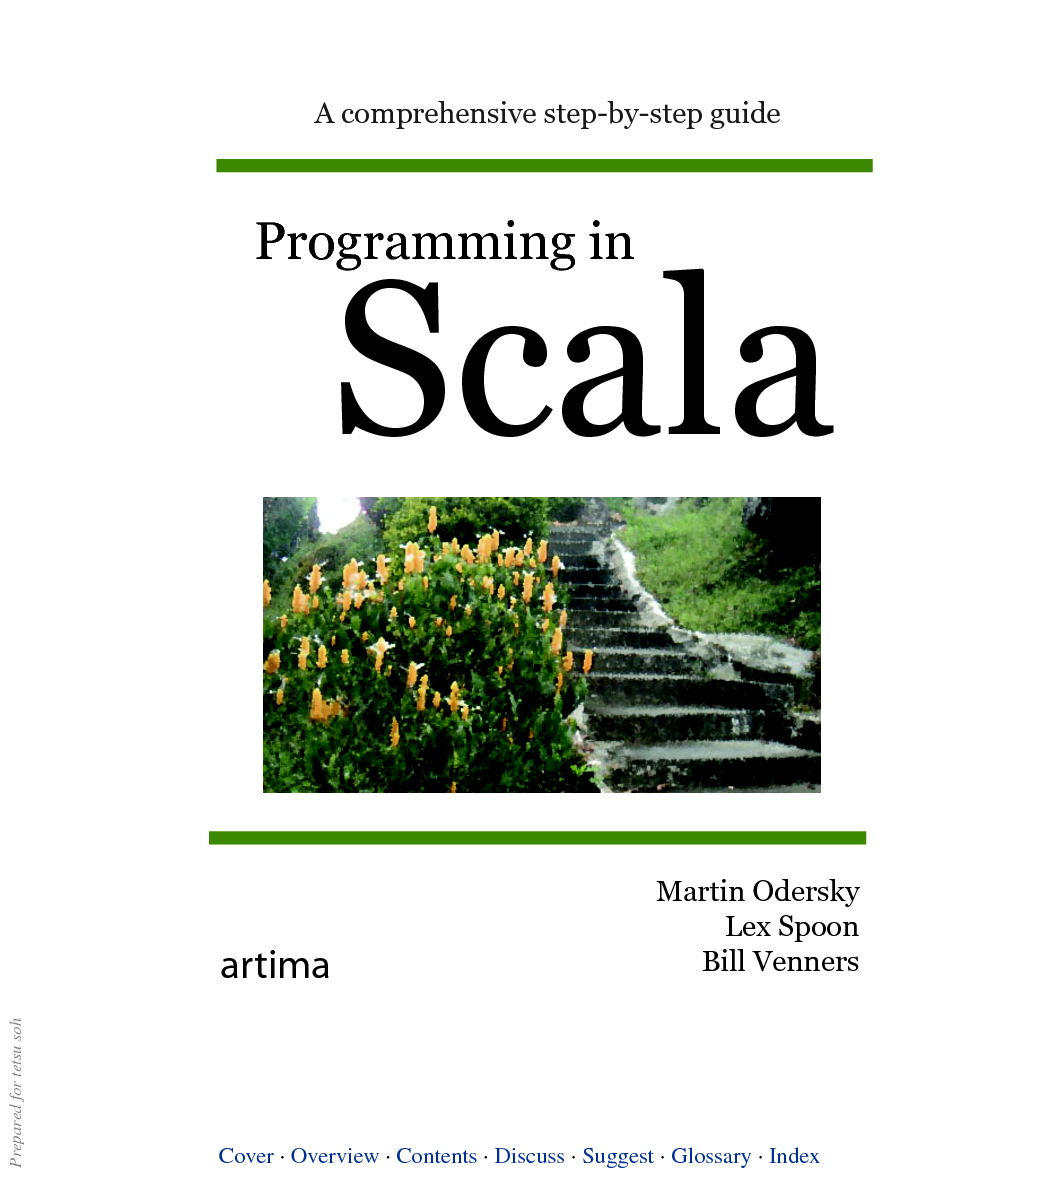
\includegraphics[width=0.5\textwidth]{resources/ProgrammingInScala.png}
\end{center}
\end{frame}
\begin{frame}{Literature}
\begin{center}
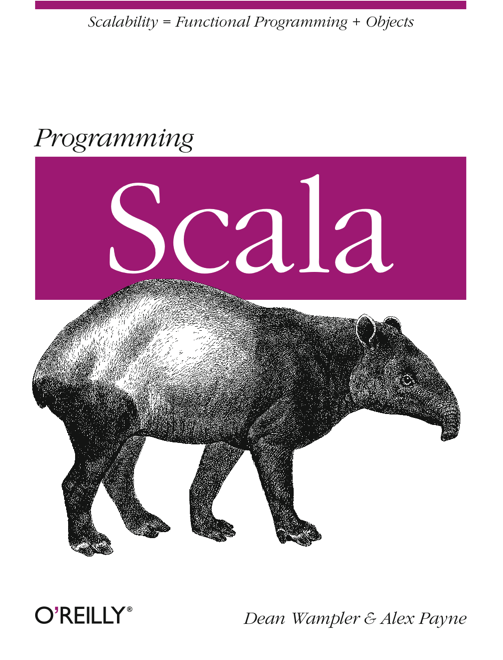
\includegraphics[width=0.5\textwidth]{resources/ProgrammingScala.png}
\end{center}
\end{frame}

\begin{frame}{Literature}
\begin{center}

\includegraphics[width=0.5\textwidth]{resources/GrundkursScala.jpg}
\end{center}
\end{frame}

\begin{frame}{Literature}
\begin{center}
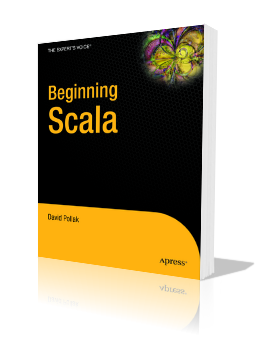
\includegraphics[width=0.5\textwidth]{resources/BeginningScala.png}
\end{center}
\end{frame}

\begin{frame}{Literature}
\begin{center}
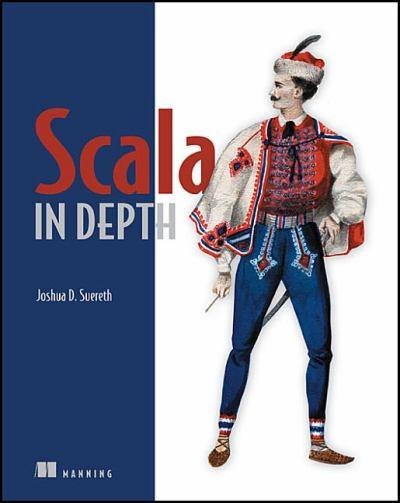
\includegraphics[width=0.5\textwidth]{resources/ScalaInDepth.jpg}
\end{center}
\end{frame}

\begin{frame}{Literature}
\begin{center}
\link{http://twitter.github.com/effectivescala/}{Effective Scala}
\end{center}
\begin{center}
\link{http://www.scala-lang.org/node/959}{and many more}
\end{center}
\end{frame}

\section{Summary}
\begin{frame}{Summary}
\begin{itemize}
  \item Scala's \highlight{community} is growing really fast
  \item Scala is \highlight{well-represented} on the web
  \item According to \highlight{Stackoverflow} and \highlight{GitHub} Scala is
  in demand
  \item Both \highlight{eclipse} and \highlight{IDEA} support Scala
  \item The \highlight{Typesafe Stack} gets you up and running in no time
  \item Scala's awesome \highlight{test frameworks} work with Java as well
  \item Scala is well-represented in \highlight{print media}
\end{itemize}
\end{frame}